% !TEX root = ../main.tex
\section{Introductory Remarks}

Ethereum-compatible blockchain environments, called Layer 2s (or \layertwos)~\cite{gudgeon2019sok}, have demonstrated an ability to reduce transaction fees by 99--99.9\% while preserving the strong guarantees of integrity and availability in the underlying blockchain. The subject of this paper concerns one subcategory of \layertwo technology called an optimistic rollup. The website \textit{L2 Beat} attempts to capitalize all tokens of known value across the top 25 \layertwo projects. It finds that the top two \layertwos are both optimistic rollups, \arb and \opt, which respectively account for 50\% and 30\% of all \layertwo value---\$4B~USD at the time of writing.\footnote{\href{https://l2beat.com/scaling/tvl/}{L2 Beat}, accessed Oct. 2022.}

We will describe the working details of optimistic rollups later in this paper but here are the main takeaways: currently, rollups are faster and cheaper than Ethereum itself. However, each \layertwo is essentially an isolated environment that cannot instantly and trustlessly interact with accounts and contracts that are running on either \layerone or other \layertwos. An optimistic rollup project will typically provide a smart contract, called a validating bridge~\cite{mccorry2021sok}, that can trustlessly move ETH (and other tokens and even arbitrary messages) between \layerone and its own \layertwo. It does value transfers by locking ETH in an \layerone contract and minting the equivalent ETH (more precisely, it is a \layertwo claim on \layerone ETH) on \layertwo and assigning it to the user's \layertwo address. Later when the user requests a withdrawal, the ETH will be destroyed on \layertwo and released by the bridge back onto \layerone according to whom its new owner is on \layertwo at the time of the request. This requires the rollup to convince the \layerone bridge contract of whom the current owner of withdrawn ETH is on \layertwo. We provide details later but this process takes time: the bridge has to wait for a period of time called the dispute window. The current default is 7 days in \arb and \opt, however the filing of new disputes can extend the window. The bottom line is that users have to wait at least 7 days to draw down ETH from an optimistic rollup. 

\paragraph{Contributions.} In this paper, we compare several methods---atomic swaps and tradeable exits---for working around this limitation. While we argue workarounds cannot be done generally, some circumstances allow it: namely, when the withdrawn token is liquid, fungible, and available on \layerone and the withdrawer is willing to pay a fee to speed up the withdrawal.  While these techniques work easily between human participants that have off-chain knowledge, such as the valid state of the \layertwo, it is harder to make them compatible with \layerone smart contracts that have no ability to validate the state of \layertwo. We propose a solution using tradeable exits and prediction markets to enable an \layerone smart contract to safely accept withdrawn tokens before the dispute period is over. We fork the current version, \nitro, of the most popular optimistic rollup, \arb, made open source\footnote{\href{https://github.com/OffchainLabs/nitro}{GitHub: Nitro}} by \offchain. We implement our solution and provide measurements. \arb is a commercial product with academic origins~\cite{kalodner2018arbitrum}. Finally, we provide an analysis of how to price exits and prediction market shares.  


 
% = = = = = = = = = = = = = = = = = = = = = = = = = = = = = = = = = = = = = = = = = =

\section{Background} 

While we describe optimistic rollups as generally as possible, some details and terms are specific to \arb. 

\paragraph{Inbox.} Rollups have emerged as a workable approach to reduce fees and latency for Ethereum-based decentralized applications. In a rollup,  transactions to be executed on \layertwo are recorded in an \layerone smart contract called the inbox. Depending on the system, users might submit to the inbox directly, or they might submit to an offchain service, called a sequencer, that will batch together transactions from many users and pay the \layerone fees for posting them into the inbox. Transactions recorded in the inbox (as \texttt{calldata}) are not executed on Ethereum, instead, they are executed in a separate environment off the Ethereum chain, called \layertwo. This external environment is designed to reduce fees, increase throughput, and decrease latency. 

\paragraph{Outbox.} Occasionally (\eg every 30--60 minutes), validators on \layertwo will produce a checkpoint of the state of all contracts and accounts in the complete \layertwo according to the latest transactions and will place this asserted state (called an \rblock) in a contract on \layerone called the outbox. Note that anyone with a view of \layerone can validate that the sequence of transactions recorded in the inbox produces the asserted \rblock in the outbox. This includes Ethereum itself, but asking it to validate this be equivalent to running the transactions on Ethereum. The key breakthrough is that the assertion will be posted with \textit{evidence} that the \rblock is correct so Ethereum does not have to check completely.

\paragraph{Optimistic vs. zk-rollups.} In practice, two main types of evidence are used. In zk-rollups,\footnote{zk stands for zero-knowledge, a slight misnomer: succinct arguments of knowledge that only need to be complete and sound, not zero-knowledge, are used~\cite{Mei21}.} a succinct computational argument that the assertion is correct is posted and can be checked by Ethereum for far less cost than running all of the transactions. However the proof is expensive to produce. In optimistic rollups, the assertions are backed by a large amount of cryptocurrency acting as a fidelity bond. The correctness of an \rblock can be challenged by anyone on Ethereum and Ethereum itself can decide between two (or more) \rblocks for far less cost than running all of the transactions (by having the challengers isolate the exact point in the execution trace where the \rblocks differ). It will then reallocate the fidelity bonds to whoever made the correct \rblock. If an \rblock is undisputed for a window of time (\eg 7 days), it is considered final.

\paragraph{Bridge.} A final piece of the \layertwo infrastructure is a bridge, which can move ETH, tokens, NFTs, and even arbitrary messages, between \layerone and \layertwo. For now, we limit the discussion to bridging ETH but the ideas extend to other tokens. If Alice has ETH on Ethereum, she can submit her ETH to a bridge smart contract on Ethereum which will lock the ETH inside of it, while generating the same amount of ETH in Alice's account inside the \layertwo environment. The bridge does not need to be trusted because every bridge operation is already fully determined by the contents of the inbox. Say that Alice transfers this ETH to Bob's address on \layertwo. Bob is now entitled to draw down the ETH from \layertwo to \layerone by submitting a withdrawal request using the same process as any other \layertwo transaction---\ie placing the transaction in the inbox on \layerone, having it executed on \layertwo, and seeing it finalized in an \rblock on \layerone. Optimistically, the \rblock is undisputed for 7 days and is finalized. Bob can now ask the bridge on \layerone to release the ETH to his address by demonstrating his withdrawal (called an exit) is included in the finalized \rblock (\eg with a Merkle-proof).

\subsection{Related Work} 

Arbitrum is first described at \textit{USENIX Security}~\cite{kalodner2018arbitrum}. Gudgeon \etal provide a systemization of knowledge (SoK) of Layer 2 technology (that largely predates rollups)~\cite{gudgeon2019sok}. McCorry \etal provide an SoK that covers rollups and validating bridges~\cite{mccorry2021sok}, while Thibault \etal provide a survey specifically about rollups~\cite{Tre22}. Some papers implement research solutions on Arbitrum for improved performance:  decentralized order books~\cite{moosavi2021lissy} and secure multiparty computation~\cite{demirag2021absentia}. The idea of tradeable exits predates our work but is hard to pinpoint a source (our contribution is implementation and adding hedges). Further academic work on optimistic rollups and bridges is nascent---we anticipate it will become an important research area.  

Other related topics are atomic swaps and prediction markets. Too many papers propose atomic swap protocols to list here but see Zamyatin \etal for an SoK of the area (and a new theoretical result)~\cite{zamyatin2021sok}. Decentralized prediction markets proposals predate Ethereum and include Clark \etal~\cite{clark2014decentralizing} and Truthcoin~\cite{sztorc2015truthcoin}. Early Ethereum projects \textit{Augur} and \textit{Gnosis} began as prediction markets. 

% = = = = = = = = = = = = = = = = = = = = = = = = = = = = = = = = = = = = = = = = = =

\section{Proposed Solution} 

For simplicity, we will describe a fast exit system for withdrawing ETH from \layertwo, however it works for any \layerone native fungible token (\eg ERC20) that is available for exchange on \layerone. We discuss challenges of fast exits for non-liquid/non-fungible tokens in Section~\ref{sec:nfts}. Consider an amount of 100 ETH. When this amount is in the user's account on \layerone, we use the notation 100 \ethone. When it is in the bridge on \layerone and in the user's account on \layertwo, we denote it 100 \ethtwo. When the ETH has been withdrawn on \layertwo and the withdrawal has been asserted in the \layerone outbox, but the dispute window is still open, we refer to it as 100 \ethxx. Other transitionary states are possible but not needed for our purposes.

\subsection{Design Landscape}

\begin{table}[t]
    \renewcommand{\arraystretch}{1.3}
    \centering
    
    \begin{tabular*}{0.9\textwidth}{@{\extracolsep{\fill}} llccccccccccccc}
    
    \textit{Type} &
    \textit{Example} & 
    \headrow{No trusted third party} & 
    \headrow{Within an \layerone transaction} &
    \headrow{Within an \layertwo rollup} &  
    \headrow{No griefing} &
    \headrow{No free option} & 
    \headrow{Opt-in anytime} & 
    \headrow{\layertwo-to-\layertwo} & 
    \headrow{} \\ \hline % Actual net movement from L2 to L1
    
    Normal Exit (baseline)   	& Arbitrum		&\full	&		&	&\full	&\full	&	&	&	\\ \hline
    Centralized   			& Coinbase	&	&\full		&\full	&\full	&\full	&	&\full	&	\\
    HTLC Swaps 			& Celer		&\full	&\prt		&\full	&	&	&	&\full	&	\\
    Conditional Transfers	& StarkEx		&\full	&\full		&\full	&	&	&	&	&	\\ % data quality
    Bridge Tokens 		& Hop 		&\prt	&\full		&\full	&	&\full	&	&\full	&	\\ 
    Tradeable Exits  		& This Work 	&\full	&$\sim$	&\full	&\full	&\full	&\full	&	&	\\ 
    Hedged Tradeable Exits  	& This Work	&\full	&$\sim$	&\full	&\full	&\full	&\full	&	&	\\ \hline
                                                                                        
    \end{tabular*}
    
\caption{Comparing alternatives for fast withdrawals from optimistic rollups for liquid and fungible tokens where \full~satisfies the property fully, \prt~partially satisfies the property, and no dot means the property is not satisfied. For our work, $\sim$ means we propose how to fully achieve the property but do not by default (see caveats in Section~\ref{sec:fidelity}).\label{tab:landscape}}

\end{table}

\paragraph{Centralized.} Consider Alice who has 100 \ethtwo and wants (something like) 99.95 \ethone for it. We describe a set of solutions for Alice. A centralized exchange (\eg \textit{Coinbase}, \textit{Binance}) can open a market for \ethtwo/\ethone. Alternatively, a bridge might rely on an established set of trustees to relay \layertwo actions to \layerone. This is called proof of authority; it is distributed but not decentralized (\ie not an \textit{open} set of participants).  

\paragraph{Hash Time Locked Contracts (HTLCs).} Assume Bob has 99.95 \ethone and is willing to swap with Alice. An atomic swap binds together (i) an \layertwo transaction moving 100 \ethtwo from Alice to Bob and (ii) an \layerone transaction moving 99.95 \ethone from Bob to Alice. Either both execute or both fail. HTLC is a blockchain-friendly atomic swap protocol. Its main drawback is that it also has a time window where Alice (assuming she is the first mover in the protocol) must wait on Bob, who might abort causing Alice's \ethtwo to be locked up while waiting (called the griefing problem), or might watch price movements before deciding to act (called free option problem). Bob needs to monitor both chains so he cannot be an autonomous smart contract. HTLCs work between two \layertwos.
% Example CELR cBridge

\paragraph{Conditional Transfers.} In this contract-based atomic swap, Alice uses an \layerone contract (called a registry) to record a request for payment of 99.95 \ethone (from anyone) with ID number 1337. Off-chain, she provides Bob with a signed \layertwo transaction (called a conditional transfer or CT) that (slow) withdraws 100 \ethtwo to Bob \textit{if and only if} payment 1337 has been received on the \layerone registry at the time the CT is added to the inbox; otherwise the CT reverts. The CT also expires (always reverts) after one hour. CTs have similar properties to an atomic swap except Alice gets paid on \layerone before anything happens on \layertwo. The registry check cannot work quickly between different \layertwos. 

% https://medium.com/starkware/conditional-transfers-the-key-to-interoperability-2e1de044fb65		X
% https://medium.com/starkware/starkexchange-fast-withdrawals-using-cookie-jars-88eefea6a11a	X
% https://docs.starkware.co/starkex/conditional-transfer.html								X

\paragraph{Bridge Token.} A third party creates a bridge on \layertwo that converts \ethtwo into a custom ticket that serves as a claim for \ethtwo~\cite{Whi21}. It creates an equivalent bridge on \layerone. Alice burns 100 tickets on \layertwo. Bob notices and generates a claim for \ethone on \layerone (assuming sufficient supply) in the equivalent \layerone bridge. To prevent Bob from maliciously minting tokens on \layerone that were not burned on \layertwo, he must post a fidelity bond of equal or greater value (otherwise Bob is trusted to not cause insolvency). After the 7-day dispute period, the \layerone bridge can verify Bob's actions are consistent with \layertwo and release his fidelity bond. Note that when you collapse this functionality, it is equivalent to Bob buying \ethxx from Alice for \ethone and receiving his \ethone back 7 days later. The extra infrastructure is necessary because today native bridges do not support tradeable exits. As in atomic swaps, Bob can fail to act (griefing) which is worst in this case if Alice cannot `unburn' her tokens, but there is no free option because Bob is a relay and not a recipient. 

\paragraph{Comparative Evaluation.} These solutions are compared with (hedged) tradeable exits---described next in the paper---in Table~\ref{tab:landscape}.
 
% https://medium.com/onther-tech/cross-rollup-transfer-hop-protocol-2c10ea041e23
% https://hop.exchange/whitepaper.pdf
% https://www.youtube.com/watch?v=U9UDblMPMoQ

\subsection{Tradeable Exits} 
\label{sec:tradeablexits}

Alice wants to withdraw 100 \ethtwo. Bob has 99.95 \ethone that will not use until after the dispute window. Bob also runs an \layertwo validator so he is assured that if Alice withdraws, it is valid and will eventually finalize. With a tradeable exit, the outbox allows Alice to change the recipient of her withdraw from herself to Bob. Thus Alice swaps her pending exit of 100 \ethone (which we call 100 \ethxx) for Bob's 99.95 \ethone on \layerone (note we discuss the actual difference in price in Section~\ref{sec:pricing}). After 7 days, Bob can ask the bridge to transfer the \ethone to his address, and the bridge checks the outbox to validate that Bob's address is the current owner of the exit.

In our forked bridge, Alice can transfer any of her exits that are in an \rblock (\ie an asserted \layertwo state update registered in the outbox). Technically, Bob can check the validity of the withdrawal as soon as it is in the inbox, and not wait 30-60 minutes for an \rblock. However for implementation reasons, it is easier to track an exit based on its place (\ie Merkle path) in an \rblock, rather than its place in the inbox. When we say a withdrawal is `fast,' we mean 30-60 minutes (\ie one \layertwo rollup). 

Like bridge tokens, tradeable exits can be approximated by a third party \layerone contract that does not modify the rollup. In this scenario, a two-stage withdrawal would occur. The user would specify the contract as the recipient of the exit, and the contract would specify the user as the recipient (initially). The user could then transfer ownership to a new account within the contract. Given this option, why modify the bridge/outbox of the rollup? We have two main arguments: (1) it is more efficient for the user to have the functionality natively in the bridge/outbox, which they have to interact with anyways; and (2) a user who initially request a `normal' withdrawal cannot change their mind and opt-in to a fast withdrawal---it is too late. A tradeable exit can bail out a user who withdrawals without realizing there is a 7-day dispute window (anecdotally, this is a common concern on support channels for optimistic rollups). It also lets a user who is aware decide if and when to expedite a withdrawal.

\subsection{Hedged Tradeable Exits}
\label{sec:PM}

One remaining issue with tradeable exits is how specialized Bob is: he must have liquidity in \ethone, be an active trader who knows how to price futures, and be an \layertwo validator. While we can expect blockchain participants with each specialization, it is a lot to assume of a single entity. The goal of this subsection is to split Bob into two distinct participants: one that has \ethone liquidity but does not know about \layertwo (Carol) and one that knows about \layertwo but is not necessarily an active trader on \layerone (David). The main impact of this change is that Carol can be an autonomous \layerone smart contract. 

Recall that Alice wants \ethone quickly in order to do something on \layerone with it; Carol can be that destination contract. The primary risk for Carol accepting \ethxx as if it were \ethone is that the \rblock containing the \ethxx withdrawal fails and the exit is worthless. If Alice can obtain insurance for the \ethxx that can be verified via \layerone, then Carol's risk is hedged and she could accept \ethxx. The insurance could take different forms but we propose using a prediction market.

\paragraph{Prediction markets.} A decentralized prediction market is an autonomous (\eg vending machine-esque) third party contract. Since we are insuring \layerone \ethxx, we need to run the market on \layerone (despite the fact that it would be cheaper and faster on \layertwo). Consider a simple market structure based on~\cite{clark2014decentralizing}. A user can request that a new market is created for a given \rblock. The market checks the outbox for the \rblock and its current status (which must be pending). Once opened, any user can submit 1 \ethone (for example, the actual amount would be smaller but harder to read) and receive two `shares': one that is a bet that the \rblock will finalize, called \final, and one that is a bet that the \rblock will fail, called \fail. These shares can be traded on any platform. At any time while the prediction market is open, any user can redeem 1 \final and 1 \fail for 1 \ethone. Once the dispute period is over, any user can request that the market close. The market checks the rollup's outbox for the status of the \rblock---since both contacts are on \layerone, this can be done directly without oracles or governance. If the \rblock finalizes, it offers 1 \ethone for any 1 \final (and conversely if it fails). The market always has enough \ethone to fully settle all outstanding shares.

It is argued in the prediction market literature~\cite{clark2014decentralizing} that (i) the price of one share matches the probability (according to the collective wisdom of the market) that its winning condition will occur, and (ii) the price of 1 \final and 1 \fail will sum up to 1 \ethone. For example, if \fail trades for 0.001 \ethone, then (i) the market believes the \rblock will fail with probability of 0.1\% and (ii) \final will trade for  0.999 \ethone. These arguments do not assume market friction: if the gas cost for redeeming shares is $D$ (for delivery cost), both share prices will incorporate $D$ (see Section~\ref{sec:pricing}). Lastly, prediction markets are flexible and traders can enter and exit positions at any time---profiting when they correctly identify over- or under-valued forecasts. This is in contrast to an insurance-esque arrangement where the insurer is committed to hold their position until completion of the arrangement.



%\textblue{\rblock will finalize eventually vs \rblock will finalize in seven days}


\paragraph{Hedging exits.} Given a prediction market, Alice can hedge 100 \ethxx by obtaining 100 \fail as insurance. Any autonomous \layerone contract (Carol) should be willing to accept a portfolio of 100 \ethxx and 100 \fail as a guaranteed delivery of 1 \ethone after the dispute period, even if Carol cannot validate the state of \layertwo.  

Perhaps surprisingly, this result collapses when withdrawing \ethtwo---consider Path 1 through the protocol. Alice withdraws 100 \ethtwo from \layertwo and obtains 100 \ethxx. Bob creates 100 \fail and 100 \final for a cost of 100 \ethone. Alice buys 100 \fail from Bob for a small fee. Alice gives Carol 100 \ethxx and 100 \fail and is credited as if she deposited 100 \ethone. In seven days, Bob gets 100 \ethone for his 100 \final and Carol gets 100 \ethone for her 100 \ethxx. If the \rblock fails, Bob has 0 \ethone and Carol has 100 \ethone from the 100 \fail. In both cases, Alice has a balance of 100 \ethone with Carol. 

In path 2, Alice withdraws 100 \ethtwo from \layertwo and obtains 100 \ethxx. Alice sells 100 \ethxx to Bob for 100 \ethone. Alice gives Carol 100 \ethone and is credited with a balance of 100 \ethone. In 7 days, Bob gets 100 \ethone for his 100 \ethxx and Carol has 100 \ethone. If the \rblock fails, Bob has 0 \ethone, Carol has 100 \ethone, and Alice has a balance of 100 \ethone with Carol.

Modulo differing gas costs and market transaction fees, paths 1 and 2 are equivalent. Path 2 does not use a prediction market at all, it only uses basic tradeable exits. Given this, do prediction markets add nothing to tradeable exits? We argue prediction markets still have value for a few reasons. (1) Speculators will also participate in the prediction market which gives Alice a chance for a fast exit even without Bob (an \layertwo validator). (2) If Alice withdraws a token other than ETH, the prediction market should still be set up to payout in ETH (otherwise you end up with 50 separate prediction markets for the 50 different kinds of tokens in any given \rblock). In this case, Alice can obtain \fail when Bob has no liquidity or interest in the token she is withdrawing (however Carol needs to incorporate an exchange rate risk when accepting an exit in one token and the insurance in ETH). (3) The PM can also help with NFTs and other non-liquid tokens (see Section~\ref{sec:nfts}).

Three of the most common types of traders are utility traders, speculators, and dealers~\cite{Har03}. With a prediction market, Alice is a utility trader and Bob is a dealer. However, there might exist speculators who want to participate in the market because they have forecasts about rollup technology, a given \rblock, the potential for software errors in the rollup or in the validator software, \etc Executives of rollup companies could receive bonuses in \final. Quick validators might profit from noticing an invalid \rblock with \fail or they might be betting on an implementation bug or weeklong censorship of the network. Speculators add liquidity to the prediction market which reduces transactional fees for Alice. However, speculation also brings externalities to the rollup system where the side-bets on an \rblock could exceed the staking requirements for posting an \rblock, breaking the crypo-economic arguments for the rollup. In reality, these externalities can never be prevented in any decentralized incentive-based system~\cite{FoBo19}. 

\section{Implementation and Performance Measurements} 

We run \arb \nitro test-net locally and use Hardhat~\cite{hardhatonline} for our experiments. We obtain our performance metrics using TypeScripts scripts. 

%The solution is made up of four components: (1) tradeable exits, (2) a prediction market to hedge the exit, and (3) a market to trade hedged (or unhedged) \ethxx. We implement (1) in \arb \nitro. For (2), one can use an existing decentralized prediction market (\eg \textit{Augur} or \textit{Gnosis}) however we further modify \arb \nitro to make it friendly to a prediction market that wants to learn the status of an \rblock (pending, confirmed, slashed). For (3), one can again use an existing market \textblue{but we make \ethxx friendly to external markets by realizing an ERC20 interface}. That said, \ethxx does not compose will with automated market makers (\eg \textit{Uniswap}), the predominate DeFi exchange (see Section~\ref{sec:uniswap}), so we also implement a basic offer contract for selling \ethxx.
%Section~\ref{sec:tradeablexits}

\subsection{Tradeable Exits}

\paragraph{Trading the exit directly through the bridge/outbox.} We fork the \arb \nitro outbox to add native support for tradeable exits. The modified outbox is open source, written in 294 lines (SLOC) of Solidity, and a bytecode of 6,212 bytes (increased by 1,197 bytes). The solidity code and Hardhat scripts are available in a GitHub repository.\footnote{\href{https://github.com/MadibaGroup/nitro/tree/fast-withdrawals}{GitHub:Nitro: Fast-Withdrawals.}} Our modifications include:

%the original outbox bytecode size 5,015 is bytes
\begin{itemize}
\item Adding the \texttt{transferSpender()} function which allows the exit owner to transfer the exit to any \layerone address even though the dispute period is not passed.
\item Adding the \texttt{isTransferred()} mapping which stores key-value pairs efficiently. The key of the mapping is the exit number and the value is a boolean.
\item Adding the \texttt{transferredToAddress} mapping which stores key-value pairs efficiently. The key of the mapping is the exit number and the value is the current owner of the exit.
\item Modifying the \texttt{executeTransactionImpl()} function. Once the dispute period is passed and the withdrawal transaction is confirmed, anyone can call the \texttt{executeTransaction()} function from the outbox (which internally calls the \texttt{executeTransactionImpl()}) and release the funds to the account that was specified by the user 7 days earlier in the \layertwo withdrawal request. With our modifications, this function is now enabled to release the requested funds to the current owner of the exit.
 \end{itemize}
 
To execute the \texttt{transferSpender()} function; Alice (who has initiated a withdrawal for 100 \ethtwo) has to provide variables related to her exit (\eg exit number), which she can query using the Arbitrum SDK\footnote{A typescript library for client-side interactions with Arbitrum.}, as well as the \layerone address she wants to transfer her exit to. The \texttt{transferSpender()} function then checks (1) if the exit is already spent, (2) it is already transferred, and (3) the exit is actually a leaf in any unconfirmed \rblock. If the exit has been transferred, the \texttt{msg.sender} is cross-checked against the current owner of the exit (recall exit owners are tracked in the \texttt{transferredToAddress} mapping added to the outbox). Once these tests are successfully passed, the \texttt{transferSpender()} function updates the exit owner by changing the address in the \texttt{transferredToAddress} mapping. This costs  85,945 Gwei in \layerone gas. Note that the first transfer always costs more as the user has to pay for initializing the \texttt{transferredToAddress} mapping. \texttt{transferSpender()} costs 48,810 and 48,798 Gwei in \layerone gas for the second and third transfer respectively. The \texttt{gasUed} for executing the new \texttt{executeTransactionImpl()} function is 91,418 Gwei in \layerone gas.


\paragraph{Trading the exit through an \layerone market.} We also implement and deploy an \layerone market that allows users to trade their exits on \layerone even though the dispute window is not passed (see Section \ref{sec:uniswap} for why \textit{Uniswap} is not appropriate). In addition, we add a new function to the \arb \nitro outbox, the \texttt{checkExitOwner()}, which returns the current owner of the exit. Figure~\ref{fig:marketflow} illustrates an overview of participant interactions and related gas costs. To start trading, Alice needs to lock her exit up in the market by calling the \texttt{transferSpender()} function from the outbox. Next, she can open a market on this exit by calling the \texttt{openMarket()} from the market contract and providing the ask price. The market checks if Alice has locked her exit (by calling the \texttt{checkExitOwner()} from the outbox) and only in that case a listing is created on this exit. The market would be open until a trade occurs or Alice calls the \texttt{closeMarket()} on her exit. Bob, who is willing to buy Alice's exit, calls the payable \texttt{submitBid()} function from the market contract. If the \texttt{msg.value} is equal or greater than Alice's ask price, the trade occurs; (1) the market calls the \texttt{transferSpender()} from the outbox providing Bob's address. Note that market can only do that since it is the current owner of the exit being traded, and (2) the \texttt{msg.value} is transferred to Alice.

The market and modified outbox are open source and written in 125 and 294 lines (SLOC) of Solidity respectively. The solidity code for these contracts in addition to the Hardhat scripts are available in a GitHub repository.\footnote{\href{https://github.com/MadibaGroup/nitro/tree/fast-withdrawals}{GitHub: Nitro: Fast-Withdrawals.}} Once deployed, the bytecode of the market and outbox is 5,772 and 6,264 bytes respectively.

\begin{figure}[t]
	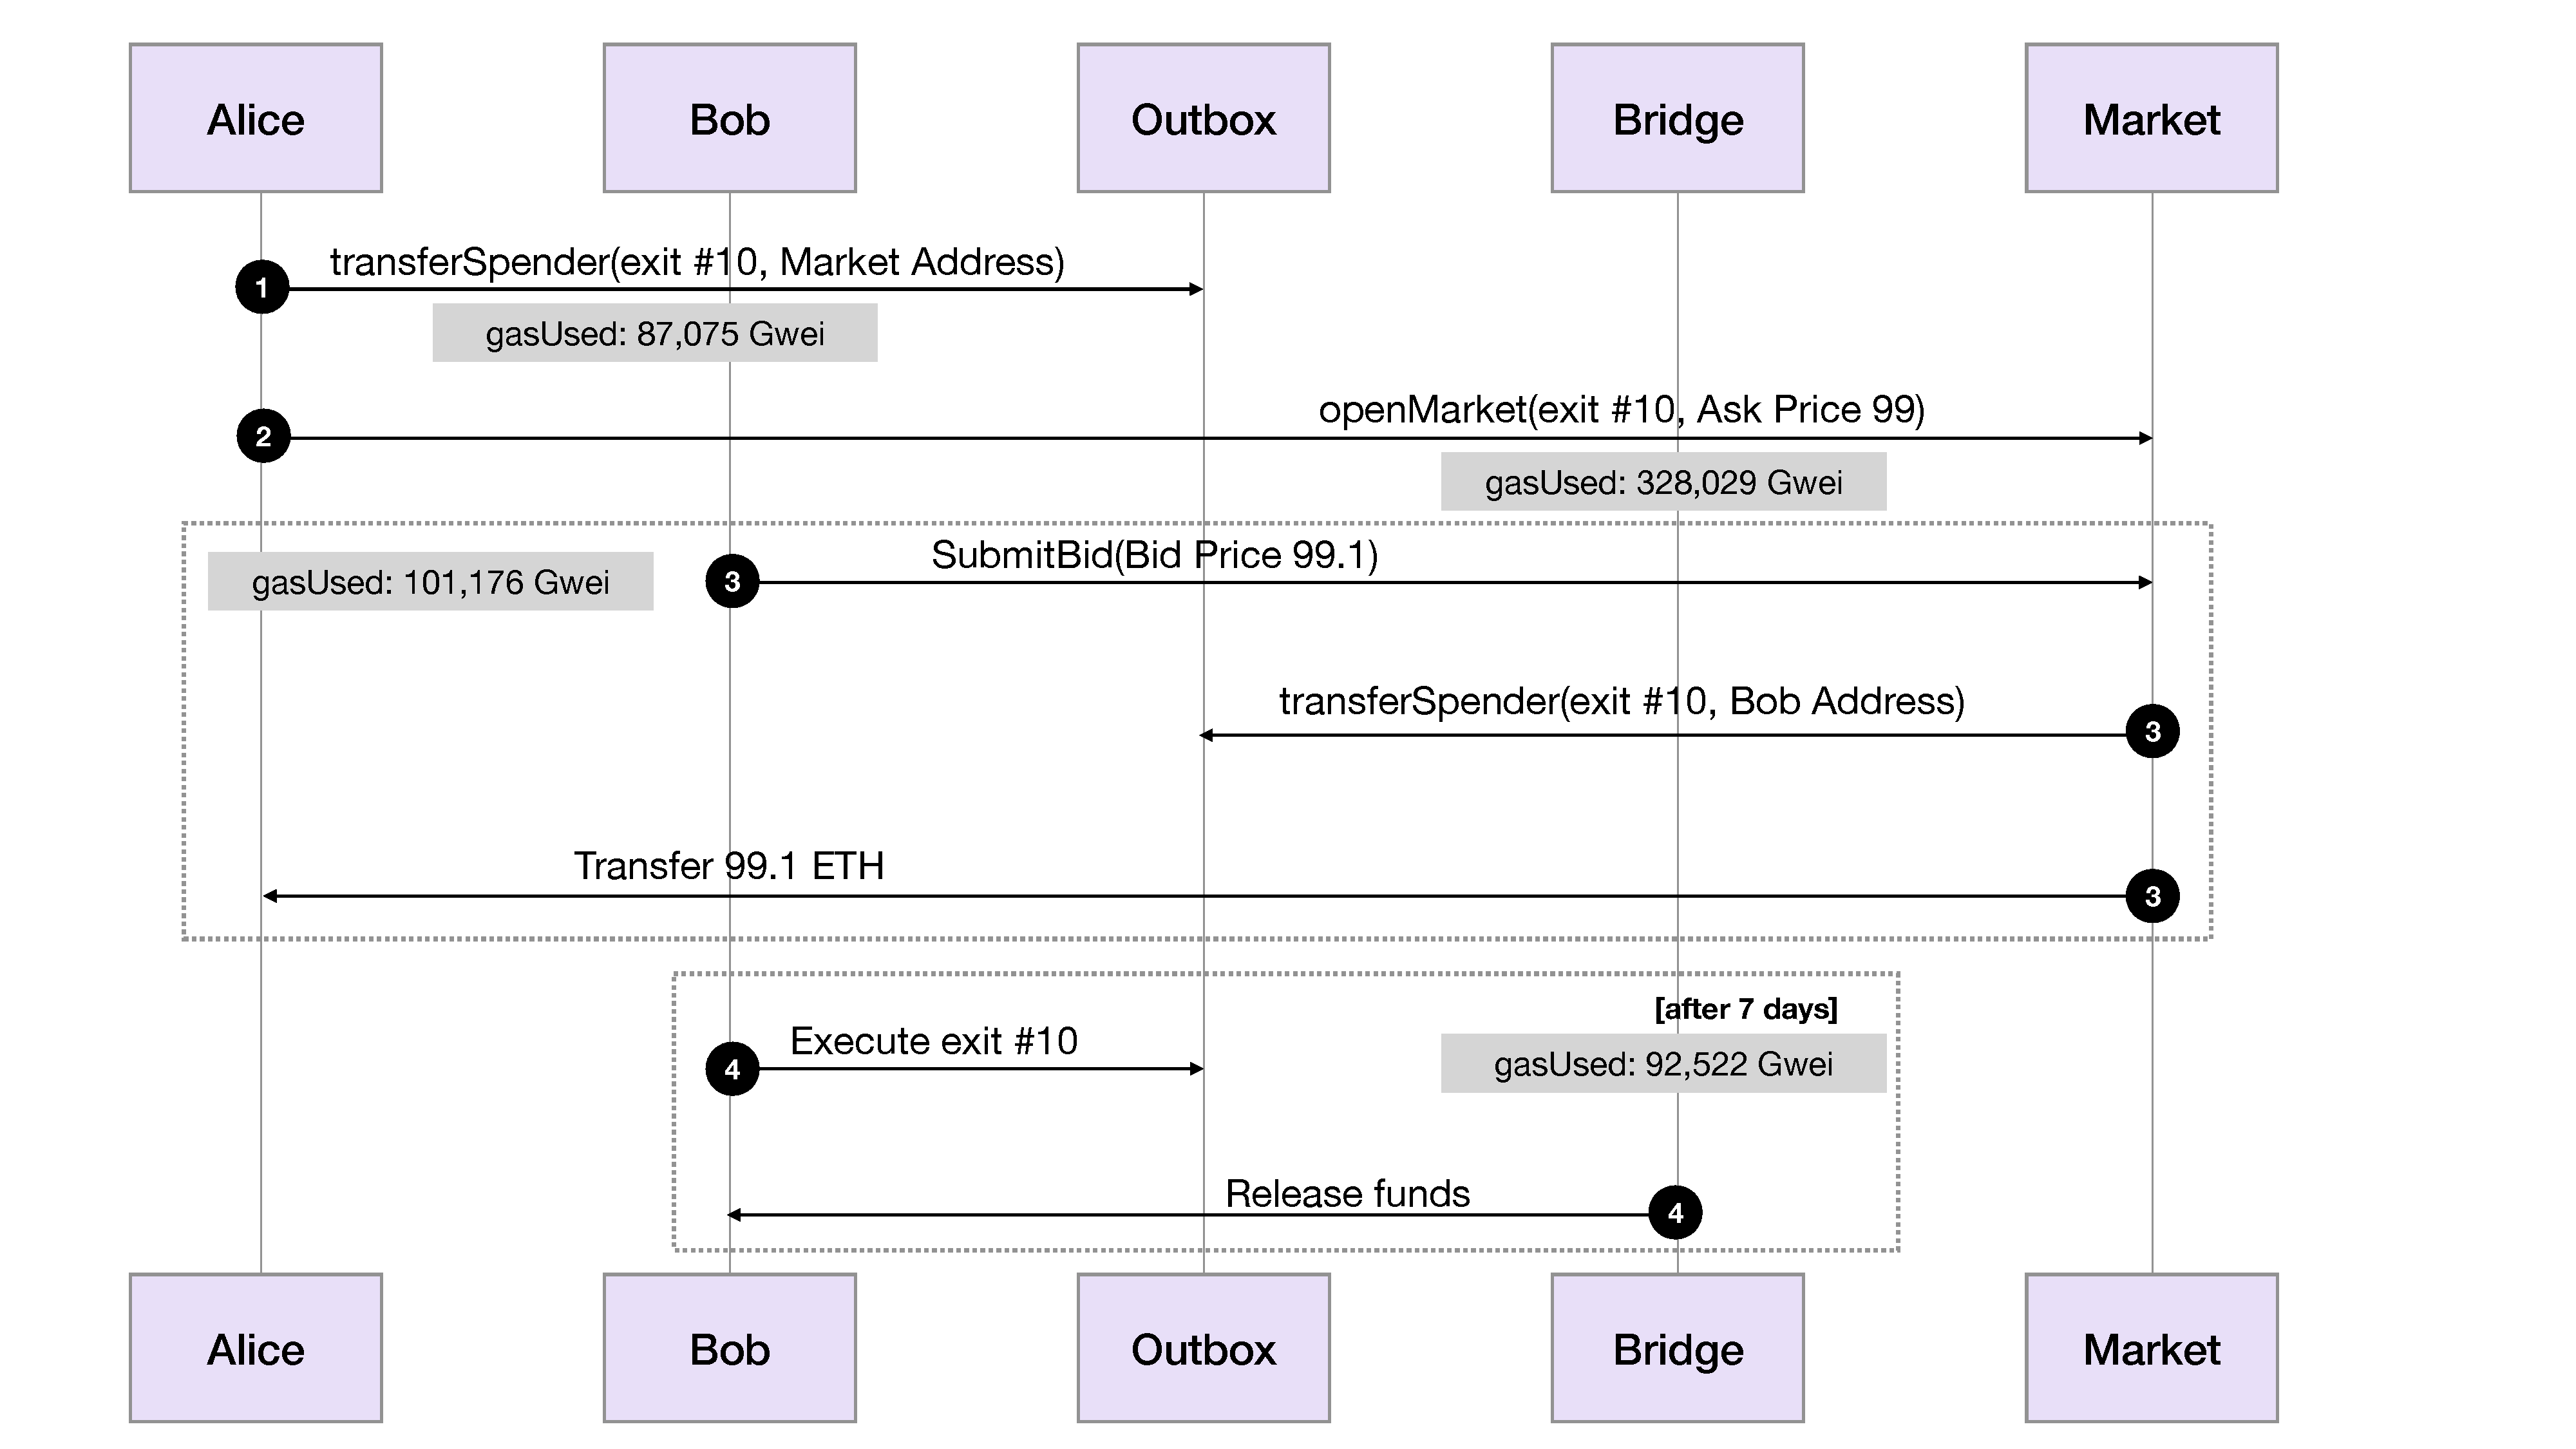
\includegraphics[width=1\textwidth]{figures/marketflow.pdf}
	\caption{Overview of trading the exit through an \layerone market.}
	\centering
	\label{fig:marketflow}
\end{figure}

\subsection{Prediction Market }
As described in Section~\ref{sec:PM}, a prediction market can be used to hedge the exit. We do not implement this as one can use an existing decentralized prediction market (\eg \textit{Augur} or \textit{Gnosis}). However, we further modify \arb \nitro to make it friendly to a prediction market that wants to learn the status of an \rblock (pending, confirmed). More specifically, we modify the \arb \nitro outbox and RollupCore smart contracts, modifications include:

\begin{itemize}
\item Adding the \texttt{assertionAtState} mapping to the outbox which stores key-value pairs efficiently. The key of the mapping is the exit number and the value is the user-defined data type \texttt{state} that restricts the variable to have only one of the \texttt{pending and confirmed} predefined values.
\item Adding the \texttt{markAsPending} function to the outbox which accepts an \rblock and marks it as pending in the \texttt{assertionAtState} mapping.
\item Adding the \texttt{markAsConfirmed} function to the outbox which accepts an \rblock and marks it as confirmed in the \texttt{assertionAtState} mapping.
\item Modifying the \texttt{createNewNode()} function in the RollupCore contract. To propose an \rblock, the validator acts through the RollupCore contract by calling a \texttt{createNewNode()} function. We modify this function to call the \texttt{markAsPending()} from the outbox which marks the \rblock as pending.
\item Modifying the \texttt{confirmNode()} function in the RollupCore contract. Once an \rblock is confirmed, the validator acts through the RollupCore contract via \texttt{confirmNode} to move the now confirmed \rblock to the outbox. We modify this function to call the \texttt{markAsConfirmed()} from the outbox which marks the \rblock as confirmed.
\end{itemize}

The modified outbox and RollupCore are open source and written in 297 and 560  lines (SLOC) of Solidity respectively. The solidity code for these contracts in addition to the Hardhat scripts are available in a GitHub repository.\footnote{\href{https://github.com/MadibaGroup/nitro/tree/fast-withdrawals}{GitHub:Nitro: Fast-Withdrawals.}} Once deployed, the bytecode of the outbox and RollupCore is 6,434 and 3,099 bytes respectively.




%
%\begin{itemize}
%\item Arbitrum's Nitro. Bridge: inbox, sequencer, outbox.
%\item Implemented a market, following is the gas cost related to the market:
%gasUsed for opening a market on an exit: 328,029
%gasUsed for transferring the exit to the market:  86,701 (it was the first transfer so a bit more expensive that the 2nd, 3rd,.. see below)
%Gas cost for submitting the Bid for when the Bid is greater than ask -> trade occurs and settles in one single submitBid tx:  105,287
%Gas cost for execution is: 92,148
%\item Modify outbox to allow tradeable exits
%\item Modify the Nitro codebase (arbnode and validator) to shrink the fraud proof window from 7 days to 1 minute: (1) Modify the confirmPeriod variable in the arbnode/node.go file, (2) modify the MakeAssertionInterval variable validator/staker.go
%\item To make the bridge prediction market friendly: 
%Modify the outbox: (1) added a Mapping that maps the proposed arbitrum block number (also known as assertion and node) to the pending state. (2) added a function which accepts a proposed block number and adds it to the pending assertions mapping.
%Modify the rollupcore: The validator acts through the RollupCore.sol contract when making an assertion by calling a createNewNode() function. We modify this function so that every time a node is created by the validator it's also added to the outbox's pending assertions mapping (outbox.addToPendingAssertions(latestNodeCreated()))
%
%\item L1 gas costs: new function (transferSpender) : 
%First Transfer: 
%1) Alice withdraws ETH from L2
%2) She transfers her exit to Bob
%transferSpender in this case costs : gasUsed : 85,945
%Second Transfer: 
%2) Now Bob transfer his exit to Carol
%transferSpender in this case costs : gasUsed : 48,810
%Third Transfer:
%2) Now Carol transfer his exit to Nancy
%transferSpender in this case costs : gasUsed : 48,798
%
% (difference of two mappings)
%
%\item L1 gas costs: execute the exit: 91,418
%
%\item Unit tests: say something
%\item What happens when an assertion fails? (pro: ticket fails with assertion, better for prediction markets (betting on assertion which is a batch of exits); ticket passes even if assertion fails, sounds better (caveat: probably won't happen)
%\item Challenges: SDK, where to change, unit test failed assertions (good assertion, bad assertion where withdrawal is ok, bad assertion where the withdrawal is problematic)
%\item Expose assertion failures/successes to external contract (submit ID for assertion, get back status: pending, finalized, or discarded). Write down the SDK call. (what happens to a failed assertions???)
%\end{itemize}


% = = = = = = = = = = = = = = = = = = = = = = = = = = = = = = = = = = = = = = = = = =


\section{Pricing}  
\label{sec:pricing}

\paragraph{Pricing \ethxx.}

Consider how much you would pay for 100 \ethxx (finalized in 7 days = 168 hours) in \ethone today. Since \ethxx is less flexible than \ethone, it is likely that you do not prefer it to \ethone, so our intuition is that it should be priced less (\eg 100 \ethxx = 99 \ethone). However, our solution works for any pricing and we can even contrive corner cases where \ethxx might be worth more than \ethone by understanding the factors underlying the price. 

In traditional finance~\cite{hull2013fundamentals}, forward contracts (and futures, which are standardized, exchange traded forwards) are very similar to \ethxx in that they price today the delivery of an asset or commodity at some future date. One key difference is that with a forward contract, the price is decided today but the actual money is exchanged for the asset at delivery time. When \ethxx is sold for \ethone, both price determination and the exchange happen today, while the delivery of \ethone for \ethxx happens in the future. The consequence is that we can adapt pricing equations for forwards/futures, however, the signs (positive/negative) of certain terms need to be inverted. 

We review the factors~\cite{hull2013fundamentals} that determine the price of a forward contract ($F_0$) and translate what they mean for \ethxx:

\begin{itemize}
\item \textit{Spot price of \ethone ($S_0$):} the price today of what will be delivered in the future. \ethxx is the future delivery of \ethone, which is by definition worth 100 \ethone today. 
\item \textit{Settlement time ($\Delta t$):} the time until the exit can be traded for \ethone. In \arb, the time depends on whether disputes happen. We simplify by assuming $\Delta t$ is always 7 days (168 hours) from the assertion time. A known fact about forwards is that $F_0$ and $S_0$ converge as $\Delta t$ approaches 0. 
\item \textit{Storage cost ($U$):} most relevant for commodities, receiving delivery of a commodity at a future date relieves the buyer of paying to store it in the short-term. Securing \ethxx and securing \ethone is identical in normal circumstances, so not having to take possession of \ethone for $\Delta t$ time does not reduce costs for a \ethxx holder. 
\item \textit{Delivery cost ($D$):} the cost of delivery of the asset, which in our case will encompass gas costs. Exchanging \ethone for \ethxx requires a transaction fee and also creates a future transaction fee to process the exit (comparable in cost to purchasing a token from an automated market maker). An \ethone seller should be compensated for these costs in the price of \ethxx.
\item \textit{Exchange rate risk:} a relevant factor when the asset being delivered is different than the asset paying for the forward. In our case, we are determining the price in \ethone for future delivery of \ethone, thus, there is no exchange risk at this level of the transaction. However, the price of gas (in the term $D$) is subject to ETH/gas exchange rates. For simplicity, we assume this is built into $D$.
\item \textit{Interest / Yield ($-r+y$):} both \ethone and \ethxx have the potential to earn interest or yield (compounding over $\Delta t$), while for other tokens, there might be an opportunity to earn new tokens simply by holding the token. Let $r$ be the (risk-free) interest (yield) rate for \ethone that cannot be earned by \ethxx, while $y$ is the opposite: yield earned from \ethxx and not \ethone. Initially $y>1$ and $r=0$, however, with \ethxx becoming mainstream, it is possible $r=y$ (especially hedged \ethxx). 
\item \textit{Settlement risk (R):} the probability that \ethone will fail to be delivered for \ethxx discounts the price of \ethxx. We will deal with this separately.

\end{itemize}

Put together, the price of \ethxx ($F_0$) is: \[ F_0 = (S_0 + U - D)\cdot e^{(-r+y)\cdot\Delta t} \cdot R \]

This value, $F_0$, is an expected value---the product of the value and the probability that the \rblock fails to finalize. However, the trader is informed because they have run verification software and checked that the \rblock validates.


\[ R = (1-\mathbf{Pr}[ \mathrm{\mathsf{rblock}~fails~to~finalize} |  \mathrm{\mathsf{rblock}~passes~software~verification} ]) \]

\paragraph{Working Example.} We start with $R$. The promise of an optimistic rollup is that it is very costly to post an \rblock that will not finalize. Assume the probability an \rblock fails for any reason is 1 in a billion. Assume the probability of inattention---that no one challenges a bad \rblock---is 1 in a million. Assume the validation software is wrong (false positive) also with 1 in a million. Using Bayes theorem, $R=(1-10^{-15})$; a near-certain probability. Next, consider the resulting price of $F_0$. Alice starts with 100 \ethxx and Bob purchases it from her. Bob can hold \ethxx with no cost ($U=0$). Alice pays the transaction fee for the deposit, however the cost for the contract for exiting \ethxx into \ethone after the dispute period is expected to be $D=0.008$ ETH ($D$). Assume a safe-ish annual percent yield (APY) on ETH deposits is 0.2\%. Assume \ethxx expires in 6 days (0.0164 years). \ethxx earns no yield ($y=0$). Plugging this into the equation, $F_0=99.665$ ETH.

As a second example, consider a smaller amount like 0.05 \ethxx (less than \$100 USD at time of writing). Now the gas costs are more dominating. $F_0=0.04186$ \ethone which is only 83.7\%. This demonstrates that fast exits are expensive for withdrawals of amounts in the hundreds of dollars.

Lastly, could \ethxx ever be worth more than \ethone? The equation says yes: with a sufficiently high $U$ or $y$. A contrived example would be some time-deferral reason (\eg tax avoidance) to prefer receiving \ethone in 7 days instead of today. However, in order to purchase \ethxx at a premium to \ethone, it would have to be cheaper to trade for it than to simply manufacture it. Someone holding \ethone and wanting \ethxx could simply move it to \layertwo and then immediately withdraw it to create \ethxx. The gas cost of this path will be one upper bound on how much \ethxx could exceed \ethone in value. 

\paragraph{Pricing \final and \fail.}

It might appear surprising at first, but one of the main results of this paper is that the price of 100 \ethxx and the price 100 \fail are essentially the same. Both are instruments that are redeemable at the same future time for the same amount of \ethone (either 100 if the \rblock finalizes and 0 if the \rblock fails) with the same probability of failure (that the \rblock fails). The carrying costs of both are identical. There may be slight differences in the gas costs of redeeming \ethone once the dispute period is over. However, the operation (at a computational level) is largely the same process. 

% = = = = = = = = = = = = = = = = = = = = = = = = = = = = = = = = = = = = = = = = = =
\section{Discussion}

\subsection{Prediction Market Fidelity}
\label{sec:fidelity}

% Buy exit before an \rblock ??? Pointer to inbox transaction ??? Pro: fast; Con: PM is for exits -> both worlds: unhedged is fast, hedged uses \rblock is PM

A prediction market that covers a larger event should attract more interest and liquidity. For example, betting on an entire \rblock will have more market interest than betting on Alice's specific exit. On the other hand, if markets are exit-specific, the market can be established immediately after Alice's withdrawal hits the inbox instead of waiting for an \rblock (hence $\sim$ in Table~\ref{tab:landscape} to indicate it could be done within one \layerone transaction). Another consideration arrises when tokens other than ETH are being withdrawn---if the payout of the market matches the withdrawn token, \fail will perfectly hedge the exit. Otherwise the hedge is in the equivalent amount of ETH which could change over 7 days. Our suggestion is to promote the most traders in a single market and avoid fragmentation---so we suggest one market in one payout currency (ETH) for one entire \rblock.

% If Alice's exit is in two \rblocks, should the prediction market cover (i) her exit in a specific \rblock or (ii) her exit regardless of the \rblock?

\subsection{Withdrawal Format}

As implemented, transferable exits can only be transferred in their entirety. If Alice wants to withdraw 100 \ethtwo and give 50 \ethxx to one person and 50 \ethxx to another, she cannot change this once she has initiated the withdraw (if she anticipates it, she can request two separate withdrawals for the smaller amounts). We could implement divisible exits and for ETH; there are no foreseen challenges since the semantics of \ethone are specified at the protocol-level of Ethereum. However for custom tokens, the bridge would need to know how divisible (if at all) a token is. In fact, a bridge should ensure that the \layertwo  behavior of the tokens is the same as \layerone (or that any inconsistencies are not meaningful). Even if a token implementation is standard, such as ERC20, this only ensures it realizes a certain interface (function names and parameters) and does not mean the functions themselves are implemented as expected (parasitic ERC20 contracts are sometimes used to trick automated trading bots.\footnote{``Bad Sandwich: DeFi Trader 'Poisons' Front-Running Miners for \$250K Profit.'' \textit{Coindesk}, Mar 2021.} The end result is that bridges today do not allow arbitrary tokens; they are built with allowlists of tokens that are human-reviewed and added by an authorized developer. In this case, ensuring divisible exits are not more divisible than the underlying token should be feasible, but we have not implemented it.

\subsection{Markets}
\label{sec:uniswap}

At the time of writing, the most common way of exchanging tokens on-chain is with an automated market maker (AMM) (\eg \textit{Uniswap}). If Alice withdraws \ethxx and Bob is a willing buyer with \ethone, an AMM is not the best market type for them to arrange a trade. AMMs use liquidity providers (LPs) who provide both token types: Alice has \ethxx but no \ethone that she is willing to lock up (hence why she is trying to fast exit). Bob has \ethone but to be an LP, he would also need to have \ethxx from another user. However, this only pushes the problem to how Bob got \ethxx from that user. The first user to sell \ethxx cannot use an AMM without locking up \ethone, which is equivalent to selling \ethxx to herself for \ethone. The second challenge of an AMM is the unlikely case that an \rblock fails and \ethxx is worthless---then the LPs have to race to withdraw their collateral before other users extract it with worthless \ethxx. It is better to use a traditional order-based market; however, these are expensive to run on \layerone~\cite{moosavi2021lissy}. One could do the matchmaking on \layertwo and then have the buyer and seller execute on \layerone, but this reintroduces the griefing attacks we have tried to avoid. For now, we implement a very simple one-sided market where Alice can deposit her \ethxx and an offer price, and Bob can later execute the trade against. If Alice is unsure how to price \ethxx, an auction mechanism could be used instead. 

\subsection{Low Liquidity or Non-Fungible Tokens}
\label{sec:nfts}

For tokens that have low liquidity on \layerone, or in the extreme case, are unique (\eg an NFT), fast exits do not seem feasible. All the fast exit methods we examined do not actually withdraw the original tokens faster; they substitute a functionally equivalent token that is already on \layerone. However, we can still help out with low-liquidity withdrawals. We should consider \textit{why} the user wants a fast exit. If it is to sell the token, they can sell the exit instead of the token to any buyer that is \layertwo-aware and willing to wait 7 days to take actual possession. To sell to an \layertwo-agnostic buyer, the seller can insure the exit with enough \fail to cover the purchase price. In this case, the buyer does not get the NFT if the \rblock fails but they get their money back.  


%Note that in this case, a prediction market is necessary: the claim is for one kind of token, while the \fail can be redeemed for \ethone, so it is not the case that the seller can just sell to the holder of \final.

%Another reason a user may want a fast withdrawal would be to use the token directly. For example, a user might have bought governance tokens on \layertwo because it was cheaper, but when a snap election over an emergency measure is proposed on \layerone, they realize they cannot get their tokens out of \layertwo fast enough to vote. Because the vote is contentious, other holders do not want to sell their tokens for a tradeable exit which would prevent them from voting. There is no way around this without modifying the DAO.

% Check flow: 
%An example modification could require voters to transfer their exit, returnable immediately after the election, and stake \ethone as a fidelity bond, returnable after the dispute period if the \rblock containing the exit finalizes.


%Last, an \layertwo-to-\layerone transfer could be a general message rather than a token transfer. For example, an oracle system might operate on \layertwo because it is cheaper, and then a need arises on \layerone for the oracle's data. Again, a prediction market can provide insurance for the data in an exit being incorrect through \fail.

%\subsection{Move PM to layer two???}

\section{Concluding Remarks}

This paper addresses a common `pain point' for users of \layertwo optimistic rollups on Ethereum. The 7-day dispute period prevents users from withdrawing ETH, tokens, and data quickly. Tradeable exits provide users with flexibility after they request a withdrawal. If they decide 7 days is too long, they can seek to trade their exit for \ethone or they can ask a contract to accept their \ethxx by bundling it with insurance against the failure of the \rblock---this way the contract does not have to be \layertwo-aware. While some users might still prefer the features of other withdrawal methods (centralized exchanges or solution like \textit{Hop}), it is useful to make the native rollup functionality as flexible as possible, especially for users who do not realize that a withdrawal induces a 7-day waiting period until it is too late. 



